\documentclass[11pt]{article}

\usepackage{thumbpdf, amssymb, amsmath, amsthm, microtype,
	    graphicx, verbatim, listings, color, fancybox}
\usepackage[pdftex]{hyperref}
%\usepackage[margin=1in]{geometry}
\usepackage{cawsty}
\usepackage{fullpage}
\usepackage{pseudocode}
\usepackage{verbatim}
\usepackage{multicol}

\usepackage{fancybox}
\usepackage{tikz}

\newcommand{\tlg}{\text{lg}}
\newcommand{\tln}{\text{ln}}
\newcommand{\tlog}{\text{log}}

\usepackage{algorithm}
%\usepackage{algorithmic}
\usepackage{amsmath}
\usepackage{amsthm}
\usepackage{algpseudocode}
\usepackage{algorithmicx}% http://ctan.org/pkg/algorithmicx
\usepackage{lipsum}% http://ctan.org/pkg/lipsum
\usepackage{xifthen}% http://ctan.org/pkg/xifthen
\usepackage{needspace}% http://ctan.org/pkg/needspace
\usepackage{hyperref}% http://ctan.org/pkg/hyperref

\usepackage{tikz}
\usetikzlibrary{arrows,%
                shapes,positioning}

\tikzstyle{vertex}=[circle,fill=black!25,minimum size=20pt,inner sep=0pt]
\tikzstyle{selected vertex} = [vertex, fill=red!24]
\tikzstyle{edge} = [draw,thick,-]
\tikzstyle{weight} = [font=\small]
\tikzstyle{selected edge} = [draw,line width=5pt,-,red!50]
\tikzstyle{ignored edge} = [draw,line width=5pt,-,black!20]

\allowdisplaybreaks[1]

% ================ ALGORITHM ENVIRONMENT ================
\newcounter{numberedAlg}% Algorithm counter
\newenvironment{numberedAlg}[1][]%
  {% \begin{numberedAlg}[#1]
    \needspace{2\baselineskip}% At least 2\baselineskip required, otherwise break
    \noindent \rule{\linewidth}{1pt} \endgraf% Top rule
    \refstepcounter{numberedAlg}% For correct reference of algorithm
    \centering \textsc{Algorithm}~\thenumberedAlg%
    \ifthenelse{\isempty{#1}}{}{:\ #1}% Typeset name (if provided)
  }{% \end{numberedAlg}
  \noindent \rule{\linewidth}{1pt}% Bottom rule
  }%

%\setlength{\parindent}{0pt}

\linespread{1.2}

\begin{document}
\cawtitle{4005-800 Algorithms}{Homework 6}

\begin{prob}{1 - 16.1-2}

Suppose that instead of always selecting the first activity to finish, we instead select the last activity to start that is compatible with all previously selected activities. Describe how this approach is a greedy algorithm, and prove that it yields an optimal solution.
\end{prob}
\begin{sol}

By definition, greedy algorithms always make a locally optimal choice at each iteration, without considering any future effects of the choice. Now, let our approach be to select the last activity to start that is compatible with all previously selected activities. We can see that this new approach is the same as choosing a single activity with the latest start time, reducing the set of compatible activities to a single subproblem based on this selection, and then repeating the selection process based on this new subset until no more activities remain. Thus, since the choice of activity is based solely on what activity has the latest start time and does not consider the future effects of this choice, we can conclude that this is a greedy algorithm. 

We can also show that this approach yields an optimal solution. Consider, for example, any non-empty subsequence of activities $S' = <a_1, a_2, ..., a_n>$, which is in monotonically decreasing order based on start times (note that this is for convenience, and we could easily continue to work with a subsequence of activities that is in monotonically increasing order based on finish times). We now prove that the largest set of compatible activities for $S'$ is $1 + $(the largest set of compatible activities in $<a_2, a_3,..., a_n>$). In other words, $a_1$ is included in some maximum-size subsequence of mutually compatible activities of $S'$.

\begin{proof}
Let $A$ be the largest set of mutually compatble activities in $S'$, and let $a_j$ be the activitiy with the latest start time. If $a_j = a_1$, then the result follows immediately. If $a_j \not= a_1$, then consider $A' = (A - \{a_j\}) \cup \{a_1\}$. Note that $A'$ is a mutually compatible set of activities since $s_1 \geq s_j$. That is, there is more time before $a_1$, and by picking $a_j$ there is nothing after (since $a_j$ has the latest start time). Now, since $|A'| = |A|$, the result follows immediately.
\end{proof}

Thus, as a direct result of this theorem, we can repeatedly choose the activity with the latest start time first, keep only those remaining activities that are compatible with this choice, and then repeat the selection process until no more compatible activities are available. This will yield a maximally sized subset of compatible activities, and since this is exactly what this new approach describes, we conclude that this is an optimal solution to the activity selection problem.

%TODO: should more be added?

\end{sol}

\begin{prob}{2 - 26.1-4}

Let $f$ be a flow in a network, and let $\alpha$ be a real number. The \textbf{scalar flow product}, denoted $\alpha f$, is a function $V \times V \to \mathbb{R}$ defined by
\begin{eqnarray*}
(\alpha f)(u,v) = \alpha \times f(u,v)
\end{eqnarray*}
Prove that the flows in a network form a \textbf{convex set}. That is, show that if $f_1$ and $f_2$ are flows, then so is $\alpha f_1 + (1 - \alpha)f_2$ for all $\alpha$ in the range $0 \leq \alpha \leq 1$.
\end{prob}
\begin{sol}

To show that flows in a network form a \textbf{convex set}, we consider the expression of scalar flow products $\alpha f_1 + (1 - \alpha)f_2$, assuming that $f_1$ and $f_2$ are valid flows in the same network. Manipulating this expression yields the following:
\begin{eqnarray}
\alpha f_1 + (1 - \alpha)f_2 & = & \alpha f_1 - \alpha f_2 + f_2 \\
& = & \alpha(f_1 - f_2) + f_2
\end{eqnarray}
Now, we consider this expression on a case-by-case basis for $\alpha$.\\

%% TODO: show substitution step explicitly instead of just assuming they can follow the math

\textbf{Case 1:} $\alpha = 0$ \\
When $\alpha = 0$, the expression $\alpha(f_1 - f_2) + f_2$ reduces to $f_2$, which is known to be a valid flow. 

\textbf{Case 2:} $\alpha = 1$ \\
When $\alpha = 1$, the expression $\alpha(f_1 - f_2) + f_2$ reduces to $f_1$, which is known to be a valid flow. 

\textbf{Case 3:} $0 < \alpha  < 1$ \\
Since $f_1$ and $f_2$ are flows, we know they satisfy the capacity constraint, skew symmetry, and flow conservation rules. Thus, we know that for all $u,v \in V$, $0 \leq f_1(u,v) \leq c(u,v)$ and $0 \leq f_2(u,v) \leq c(u,v)$. Using this relationship with the convex criteria described above yields the following lower bound for all $u,v \in V$:
\begin{eqnarray*}
\alpha f_1(u,v) + (1 - \alpha)f_2(u,v) & \geq & 0 \cdot \alpha f_1(u,v) + 0 \cdot (1 - \alpha)f_2(u,v) \\
& = & 0
\end{eqnarray*}
This is because $\alpha \geq 0$ and $1 - \alpha \geq 0$ (the sum of the two terms is positive). Similarly, we can examine the original convex criteria described above to find an upper bound for all $u,v \in V$ as follows:
\begin{eqnarray*}
\alpha f_1(u,v) + (1 - \alpha)f_2(u,v) & \leq & \alpha c(u,v) + (1 - \alpha)c(u,v) \\
& = & \alpha c(u,v) + c(u,v) - \alpha c(u,v) \\
& = & c(u,v)
\end{eqnarray*}
Thus, we see that the convex criteria expression satisfies the capacity constraint. 

We now consider this expression in terms of skew symmetry (i.e. the net flow at a vertex). Since $f_1$ and $f_2$ are flows, we know that for each pair of vertices $u, v \in V$, $f_1(u,v) = -f_1(v,u)$ and $f_2(u,v) = -f_2(v,u)$ by skew symmetry. Therefore, we know the following for each pair of vertices $u, v \in V$:
\begin{eqnarray*}
\alpha f_1(u,v) + (1 - \alpha)f_2(u,v) & = & -\alpha f_1(v,u) - (1 - \alpha)f_2(v,u) \\
& = & -(\alpha f_1(v,u) + (1 - \alpha)f_2(v,u))
\end{eqnarray*}
Thus, the original convex criteria expression satisfies the skew symmetry rule.

Now, by flow conservation, we know that for all vertices $u \in V - \{s,t\}$ we have $\sum_{v \in V}f_1(u,v) = 0$ and  $\sum_{v \in V}f_2(u,v) = 0$. Using this fact, we examine the convex critera expression described above for all vertices $u \in V - \{s,t\}$ as follows:
\begin{eqnarray*}
\sum_{v \in V}\alpha f_1(u,v) + (1 - \alpha)f_2(u,v) & = & \sum_{v \in V}\alpha f_1(u,v) + \sum_{v \in V}f_2(u,v) - \sum_{v \in V}\alpha f_2(u,v) \\
& = & \sum_{v \in V}\alpha f_1(u,v) - \sum_{v \in V}\alpha f_2(u,v) \\
& = & \alpha\sum_{v \in V} f_1(u,v) - \alpha\sum_{v \in V} f_2(u,v) \\
& = & 0
\end{eqnarray*}
Thus, since the convex critera expression $\alpha f_1(u,v) + (1 - \alpha)f_2(u,v)$ satisfies the capacity constraint, skew symmetry, and flow constraint rules in this case, we conclude that it is also a flow. Therefore, we also conclude that flows in a network form a convex set.
\end{sol}

\begin{prob}{3 - 26.2-2}

In Figure $26.1(b)$, what is the flow across the cut $(\{s, v_2, v_4\}, \{v_1, v_3, t\})$? What is the capacity of this cut?
\end{prob}
\begin{sol}
The graph in Figure $26.1(b)$ is shown below.

\begin{center}
	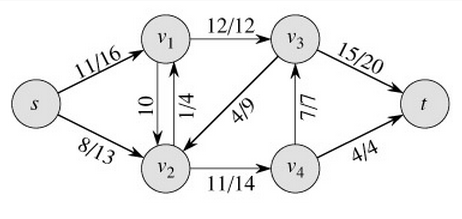
\includegraphics[width=90mm]{graphpic.png}
\end{center}

By considering the cut $(\{s, v_2, v_4\}, \{v_1, v_3, t\})$, we know the edges that cross the cut boundary are $\{(u,v) : u \in S, v \in T, (u,v) \in E\} = \{(s, v_1), (v_2, v_1), (v_3, v_2), (v_4, v_3), (v_4, t)\}$. The net flow of this $s-t$-cut is then as follows:
\begin{eqnarray*}
f(S, T) & = & f(s, v_1) + f(v_2, v_1) + f(v_3, v_2) + f(v_4, v_3) + f(v_4, t) \\
& = & 11 + 1 + (-4) + 7 + 4 \\
& = & 19
\end{eqnarray*}
Since the capacity of the cut is defined as the sum of the edge capacities from all vertices $u \in S$ to $v \in T$, we have the following capacity:
\begin{eqnarray*}
c(S, T) & = & c(s,v_1) + c(v_2, v_1) + c(v_4, v_3) + c(v_4, t) \\
& = & 16 + 4 + 7 + 4 \\
& = & 31
\end{eqnarray*}

\end{sol}

\end{document}
